\chapter{Results}
Monte Carlo for the basic environment with 4 possible actions is shown in figure \ref{fig:mcbasicfull}. The rewards were normalised so the ideal workflow every time gives a reward of 1.0. For this algorithm $\gamma=1.0$ and $\varepsilon=0.01$. It is clear from the figure that Monte Carlo works optimally: it learns quickly (levelling off within 500 episodes) and returns a high average reward. This is expected as Monte Carlo is designed to work well with episodic environments, and has a low bias.
\begin{figure}[h]
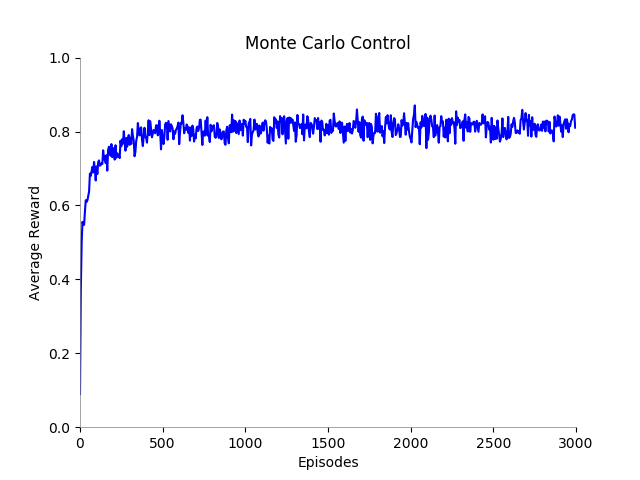
\includegraphics[width=\textwidth]{resultsbasic/21_100runs_3000_normalised}
\caption[Monte Carlo Control for Basic Environment]{Monte Carlo control averaged over 100 runs for an environment with 4 possible actions, normalised to true reward on optimal behaviour}
\label{fig:mcbasicfull}
\end{figure}

Q-learning, on the other hand, is not well suited to this environment with non-Markov states. As can be seen in figure \ref{fig:qgraph}, the algorithm levels off at a reward level of only 20\% of the true reward value. Because of such poor results for the basic environment, Monte Carlo was the main focus for the remainder of the trials.
\begin{figure}[h]
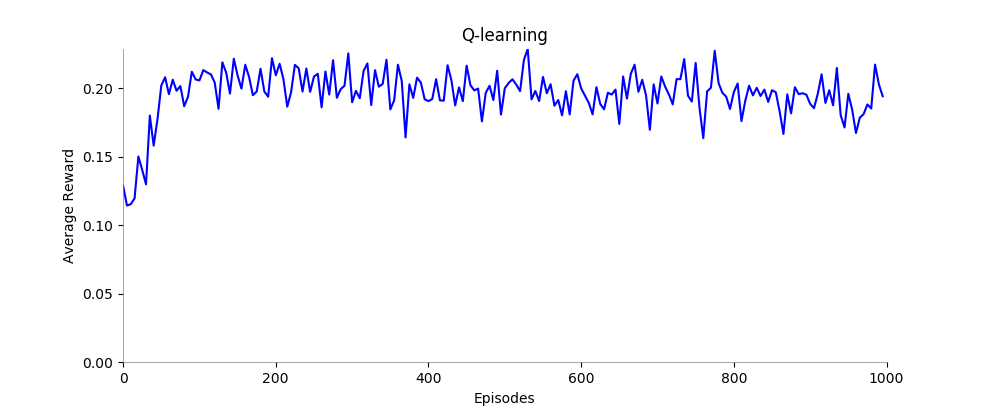
\includegraphics[width=\textwidth]{resultsq/basic10002}
\caption[Q-learning for the basic environment]{Q-learning averaged over 1000 runs for an environment with 4 possible actions, normalised to true reward}
\label{fig:qgraph}
\end{figure}

\begin{comment}
\begin{figure}[h]
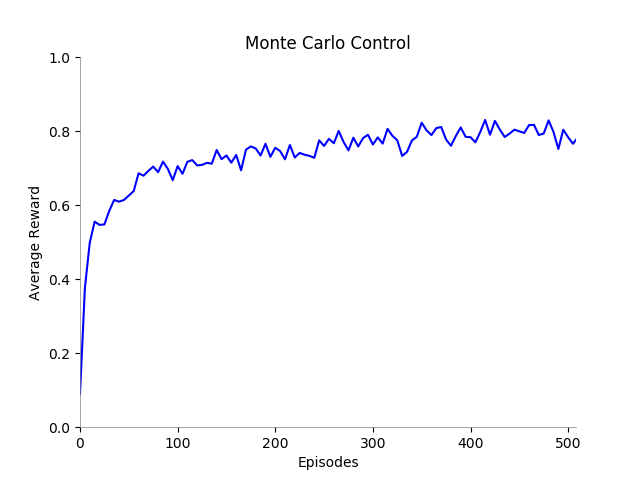
\includegraphics[width=\textwidth]{resultsbasic/21_100runs_500normalised}
\caption[Monte Carlo Control for Basic Environment]{Monte Carlo control averaged over 100 runs for an environment with 4 possible actions, normalised to true reward on optimal behaviour}
\label{fig:mcbasiczoom}
\end{figure}
\end{comment}

Figure \ref{fig:diffgammas} shows the effects of a different $\gamma$ choice. Recall from section \ref{MDP} that $\gamma\in\left(0,1\right]$ is the discount factor, and a smaller discount factor emphasises immediate reward.
\begin{figure}[h]
\centering
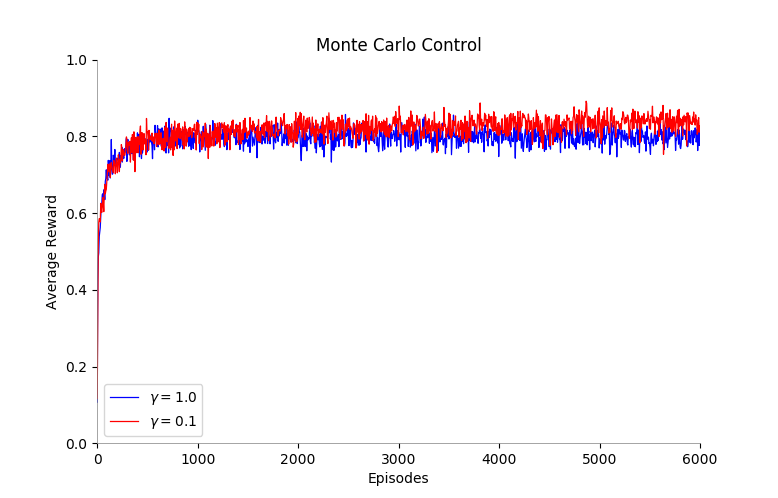
\includegraphics[width=.85\textwidth]{resultsbasic/differentgammas}
\caption[Monte Carlo Control]{Monte Carlo control averaged over 100 runs for an environment with 4 possible actions, with different choices of $\gamma$}
\label{fig:diffgammas}
\end{figure}

As the environment only provides a reward once at the end of an episode, and we are looking to find paths with the least amount of time steps, it is logical to choose a smaller discount factor (to emphasize the preference for immediate reward). Although a smaller discount factor means the algorithm learns (marginally) slower, it also means the eventual average reward is higher, and is therefore the optimal choice for an environment of this style.
\begin{figure}[h]
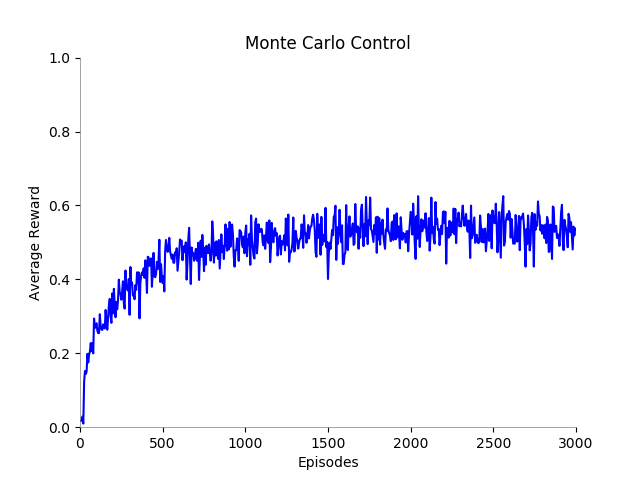
\includegraphics[width=\textwidth]{resultsdiscretemc/41100runs3000normalised}
\caption[Monte Carlo Control for Discretised Environment]{Monte Carlo control averaged over 100 runs for an environment with 20 possible actions}
\label{fig:discrete}
\end{figure}

With the action space expanded for the discretised environment, the average reward lowers as expected. In figure \ref{fig:discrete} is the Monte Carlo control for an environment that has 20 possible actions: the four original operators, with the possible values $1.0,2.0,3.0,4.0$ and $5.0$. The hidden function is still a basic two step function (this time $-1.0\times4.0$). The algorithm still achieves a good learning rate, although not as fast as the previous  
\begin{comment}
\begin{figure}[h]
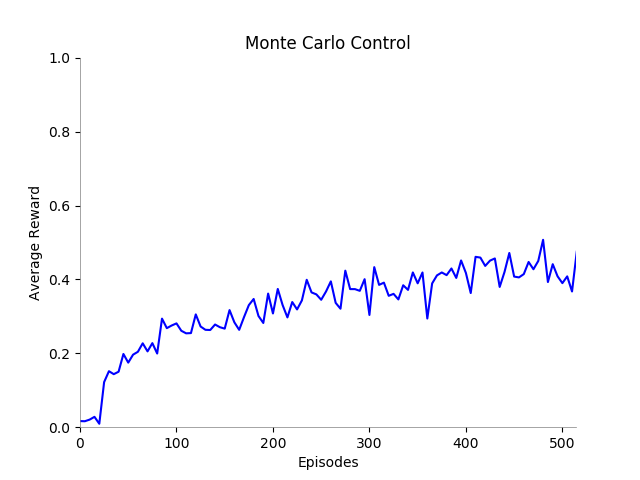
\includegraphics[width=\textwidth]{resultsdiscretemc/41_100runs500normalised}
\caption[Monte Carlo Control for Discretised Environment]{Monte Carlo control averaged over 100 runs for an environment with 20 possible actions}
\end{figure}
\end{comment}
\begin{figure}[h]
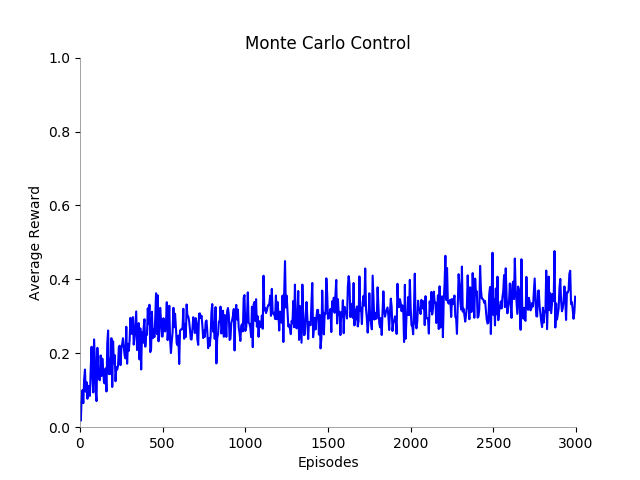
\includegraphics[width=\textwidth]{resultscomplexmc/413_100runs_3000normalised}
\caption[Monte Carlo Control for the discretised environment with complex function]{Monte Carlo control averaged over 100 runs for an environment with 20 possible actions, learning a more complex hidden function}
\end{figure}

\begin{figure}[h]
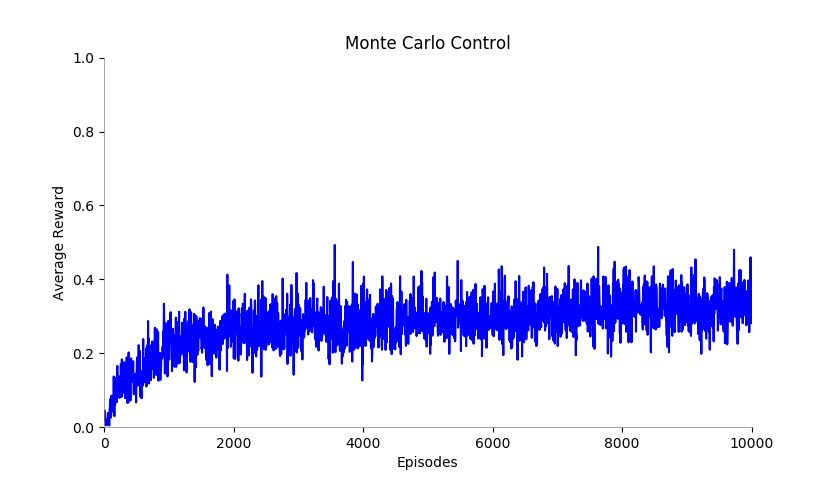
\includegraphics[width=\textwidth]{discretequarter/figure_1}
\caption[Monte Carlo Control for the discretised environment with 68 actions]{Monte Carlo control averaged over 100 runs for an environment with 68 possible actions}
\end{figure}







